\documentclass[border=2pt]{standalone}
\usepackage[utf8]{inputenc}\usepackage[T1]{fontenc}\usepackage{amsmath,tikz}\usetikzlibrary{shapes,arrows.meta,positioning}
\begin{document}
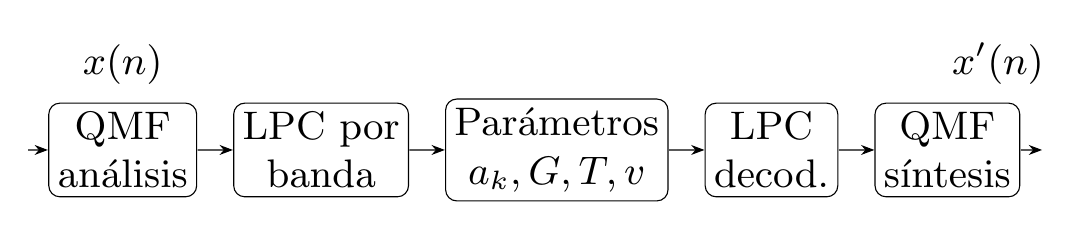
\begin{tikzpicture}[font=\small,scale=1.6,transform shape,node distance=0.28cm,blk/.style={draw,rounded corners,minimum height=0.55cm,inner sep=2pt,align=center},>=Stealth]
\node[blk](qa){QMF\\an\'alisis};
\node[blk,right=of qa](l){LPC por\\banda};
\node[blk,right=of l](p){Par\'ametros\\$a_k,G,T,v$};
\node[blk,right=of p](d){LPC\\decod.};
\node[blk,right=of d](qs){QMF\\s\'intesis};
\draw[->](-0.75,0)--(qa);\draw[->](qa)--(l);\draw[->](l)--(p);\draw[->](p)--(d);\draw[->](d)--(qs);\draw[->](qs)--++(0.75,0);
\node[above=0.02cm of qa]{$x(n)$};\node[above=0.02cm of qs,xshift=0.4cm]{$x'(n)$};
\end{tikzpicture}
\end{document}
